% ---------------------------------------------------------------------------- %

\section{Construção}
\label{cap:construcao}

Tendo-se terminado o processo de especificação do sistema, procedeu-se à sua implementação. Neste capítulo são primeiramente enumeradas as principais tecnologias utilizadas na sua construção, descrevendo-se também vários aspetos relevantes da sua implementação. É depois descrito o procedimento de instalação do sistema e apresentado brevemente o produto obtido.

% ---------------------------------------------------------------------------- %

\subsection{Tecnologias utilizadas}
\label{sec:construcao:tecnologias}

O sistema desenvolvido consiste em um servidor \emph{web}, o qual é acedido por clientes remotos através de um \emph{web browser}. Para a implementação do mesmo, utilizaram-se as seguintes principais tecnologias e \emph{frameworks}:

\begin{itemize}

    \item Sistema de gestão de bases de dados \emph{Microsoft SQL Server}\footnote{\url{https://www.microsoft.com/en-us/sql-server}, acedido a 23 de maio de 2019};

    \item \emph{Microsoft .NET Core} 2.1\footnote{\url{https://dotnet.microsoft.com/}, acedido a 23 de maio de 2019}, utilizando-se a liguagem \emph{C\#};

    \item \emph{Entity Framework Core} 2.1\footnote{\url{https://dotnet.microsoft.com/apps/aspnet}, acedido a 23 de maio de 2019};

    \item \emph{Microsoft ASP.NET Core} 2.1\footnote{\url{https://docs.microsoft.com/en-us/ef/core}, acedido a 23 de maio de 2019}, utilizando-se a arquitetura \emph{Model-View-Controller} (MVC);
    
    \item \emph{Bing Maps API}\footnote{\url{https://www.microsoft.com/en-us/maps/choose-your-bing-maps-api}, acedido a 23 de maio de 2019};
    
    \item \emph{YamlDotNet} 6.0\footnote{\url{https://github.com/aaubry/YamlDotNet}, acedido a 23 de maio de 2019}.

\end{itemize}

% ---------------------------------------------------------------------------- %

\subsection{Detalhes de implementação}
\label{sec:construcao:implementacao}

O sistema desenvolvido segue o padrão arquitetural \emph{Model-View-Controller} (MVC):

\begin{itemize}

    \item \emph{Models}: representam, gerem e persistem a informação utilizada pelo sistema;
    
    \item \emph{Views}: definem a interface gráfica disponibilizada aos utilizadores do sistema, apresentando informação gerida pelos \emph{models};
    
    \item \emph{Controllers}: gerem a interação do utilizador com a interface gráfica disponibilizada pelas \emph{views}, interatuando com os \emph{models} para obter e modificar informação.
    
\end{itemize}

A informação da aplicação é persistida numa base de dados relacional disponibilizada por uma instância de um servidor \emph{Microsoft SQL Server}. O mapeamento do modelo relacional para objetos foi implementado com recurso à plataforma \emph{Entity Framework Core}.

% ---------------------------------------------------------------------------- %

\subsection{Procedimento de instalação}
\label{sec:construcao:instalacao}

Uma vez que o sistema desenvolvido corresponde apenas a um \emph{web} server, o processo de instalação (ou \emph{deployment}) do mesmo envolve apenas intervenção por parte do administrador da máquina onde se deseja que este corra.

Por forma a se instalar o sistema, os seguintes pré-requisitos devem ser cumpridos:

\begin{itemize}

    \item A máquina onde o \emph{web} server irá correr deve utilizar alguma versão do sistema operativo \emph{Windows} com suporte para as tecnologias enumeradas na secção anterior;
    
    \item A mesma máquina deve ter acesso (local ou remoto) a uma instância de um servido \emph{Microsoft SQL Server}, no qual os dados da aplicação serão persistidos.
    
\end{itemize}

Tendo em conta que a aplicação é disponibilizada num único arquivo de ficheiros, o procedimento de instalação do sistema consiste então nos seguintes passos:

\begin{enumerate}

    \item Extrair todo os ficheiros do arquivo da aplicação;

    \item Alterar o campo \path{ConnectionStrings.DefaultConnection} do ficheiro \path{appsettings.json} por forma a corresponder à instância do servidor \emph{Microsoft SQL Server} (e base de dados nesse servidor) onde os dados da aplicação devem ser persistidos;
    
    \item Executar o programa \path{BelaSopa.exe}, o qual corresponde ao servidor \emph{web} que implementa o sistema;
    
    \item Opcionalmente, configurar o sistema operativo por forma a que este programa seja executado aquando do reinício da máquina;

    \item Garantir que eventuais configurações de rede permitam que clientes remotos acedam ao servidor \emph{web}.
    
\end{enumerate}

Uma vez concluído este processo, os clientes terão acesso ao sistema através do seu \emph{web browser}, especificando o endereço da máquina em que o servidor \emph{web} está instalado.

% ---------------------------------------------------------------------------- %

\subsection{Produto final}
\label{sec:construcao:produto-final}

As Figuras~\ref{fig:construcao:final-1} a~\ref{fig:construcao:final-4} apresentam, a título de exemplo, o aspeto final de várias interfaces representativas disponibilizadas pelo sistema \emph{Bela Sopa}.

\begin{landscape}

\begin{figure}[p]
  \centering
  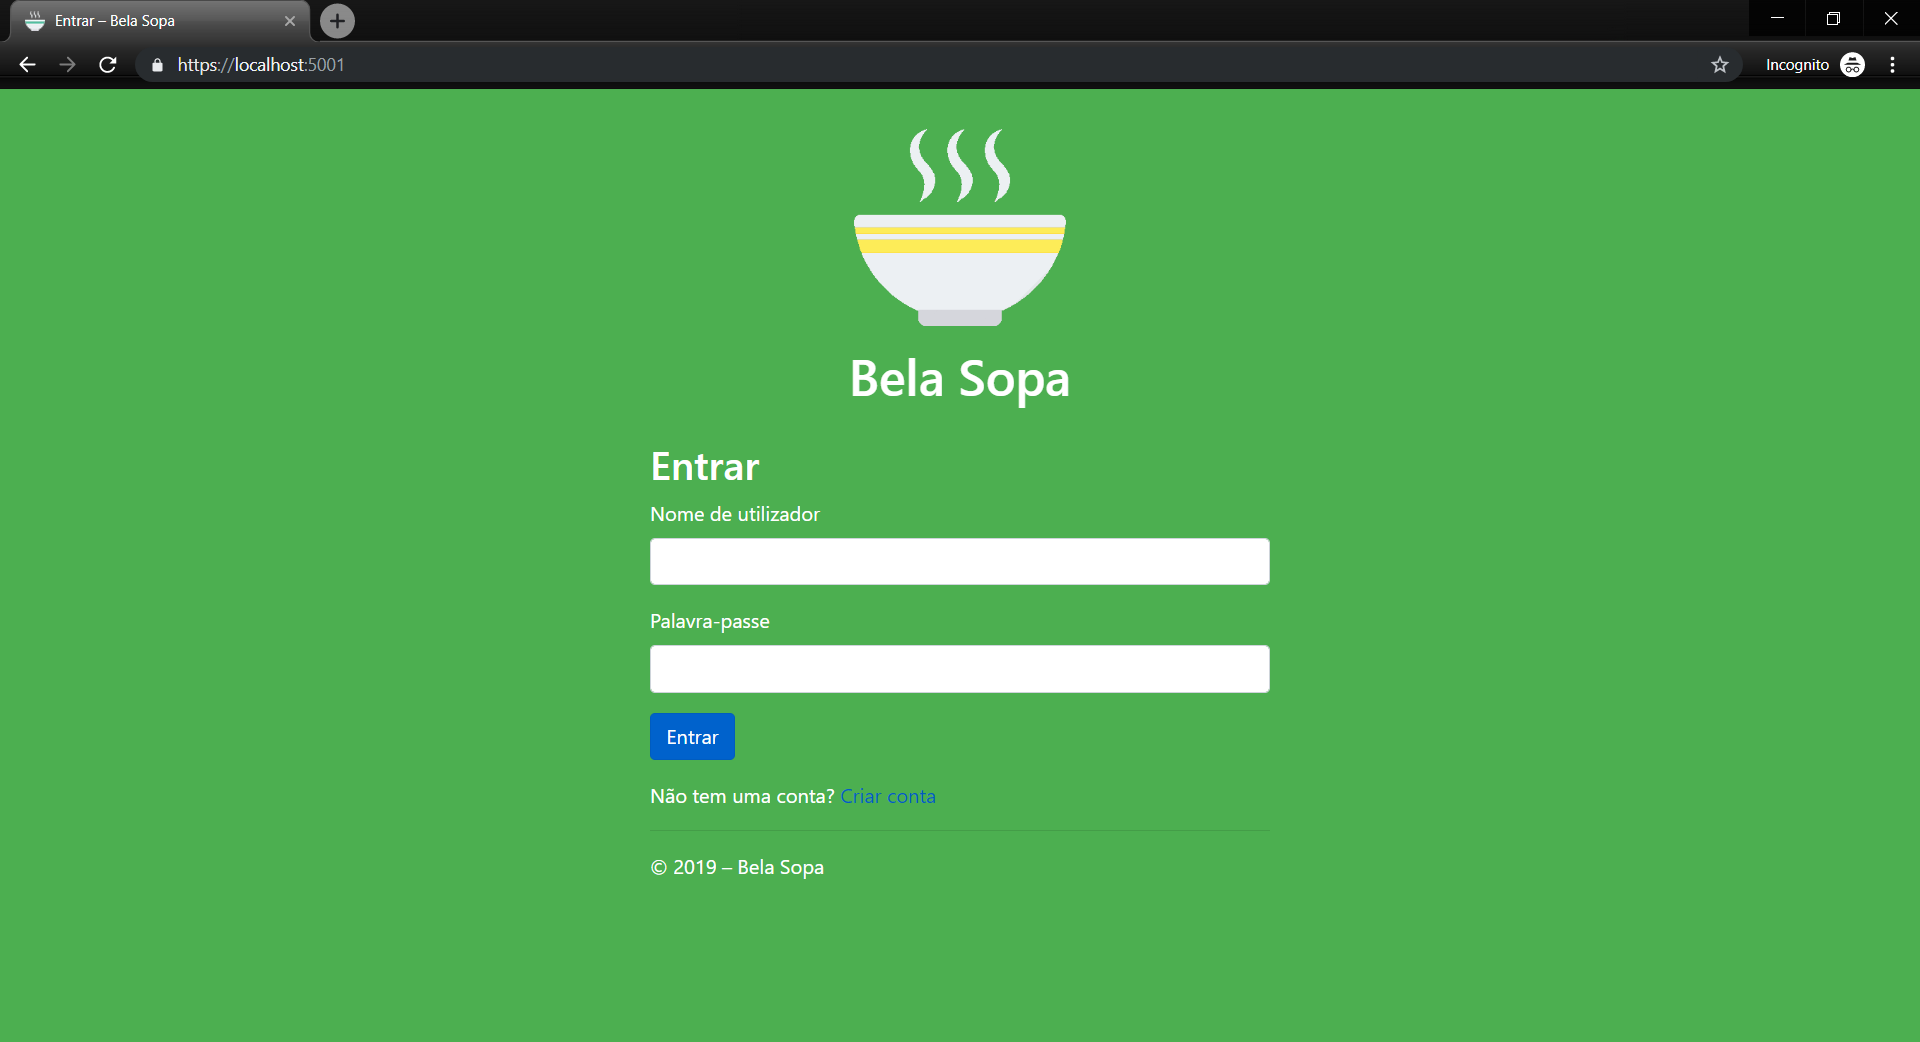
\includegraphics[height=.85\textheight]{figures/11/final-1.png}
  \caption{Aspeto final da interface de autenticação.}
  \label{fig:construcao:final-1}
\end{figure}

\begin{figure}[p]
  \centering
  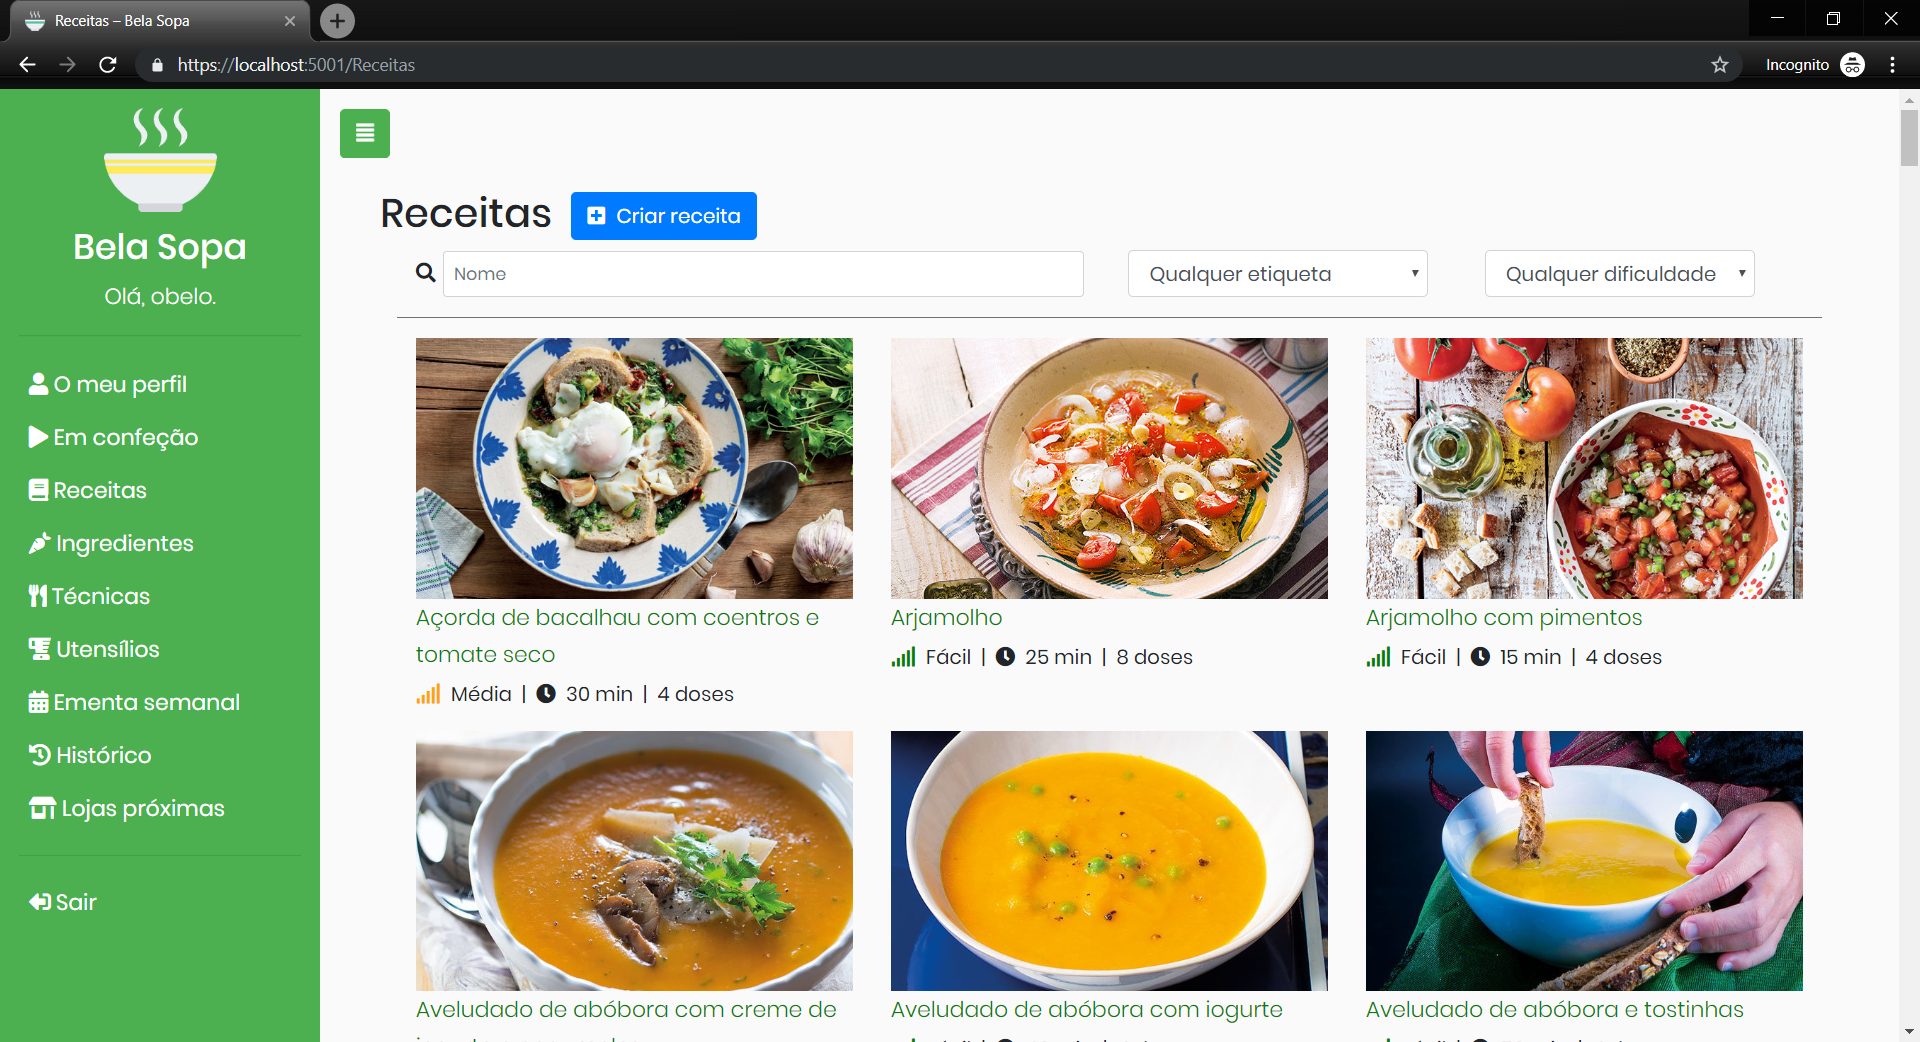
\includegraphics[height=.85\textheight]{figures/11/final-2.png}
  \caption{Aspeto final da interface de listagem de receitas.}
  \label{fig:construcao:final-2}
\end{figure}

\begin{figure}[p]
  \centering
  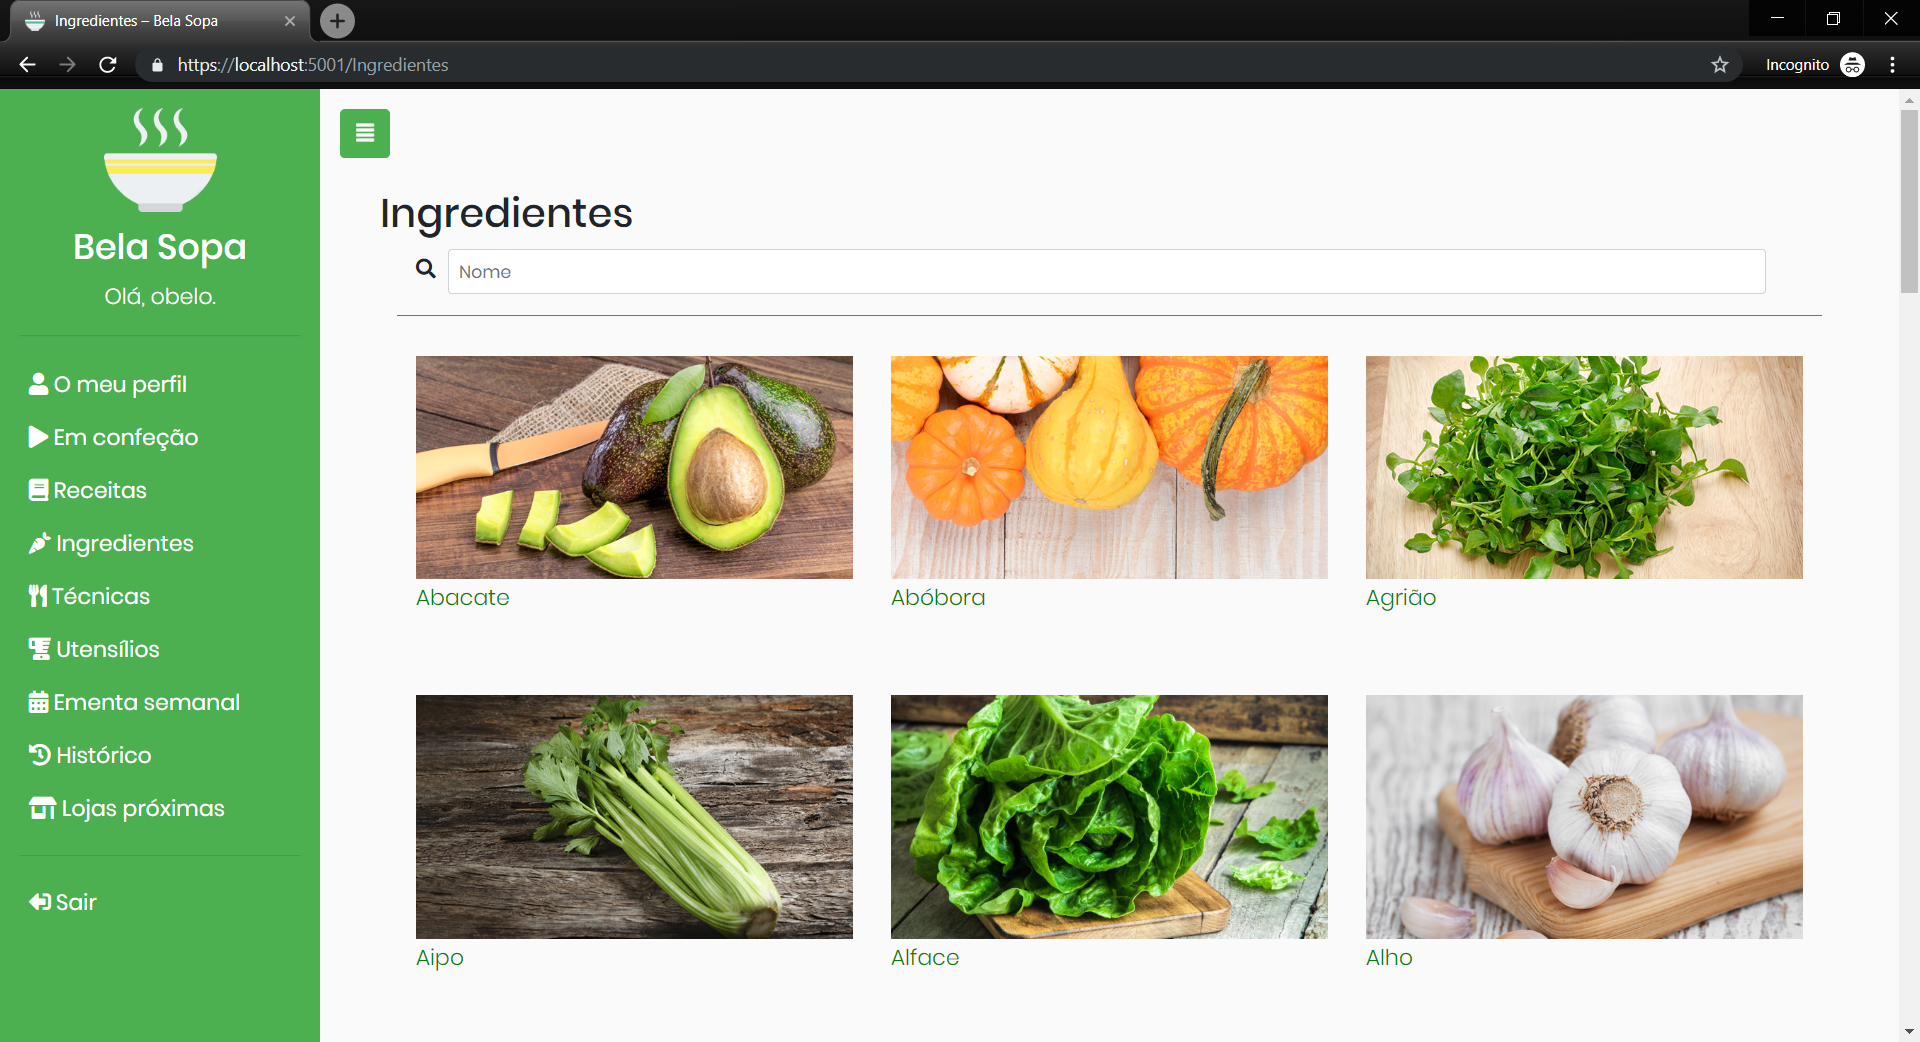
\includegraphics[height=.85\textheight]{figures/11/final-3.png}
  \caption{Aspeto final da interface de listagem de ingredientes.}
  \label{fig:construcao:final-3}
\end{figure}

\begin{figure}[p]
  \centering
  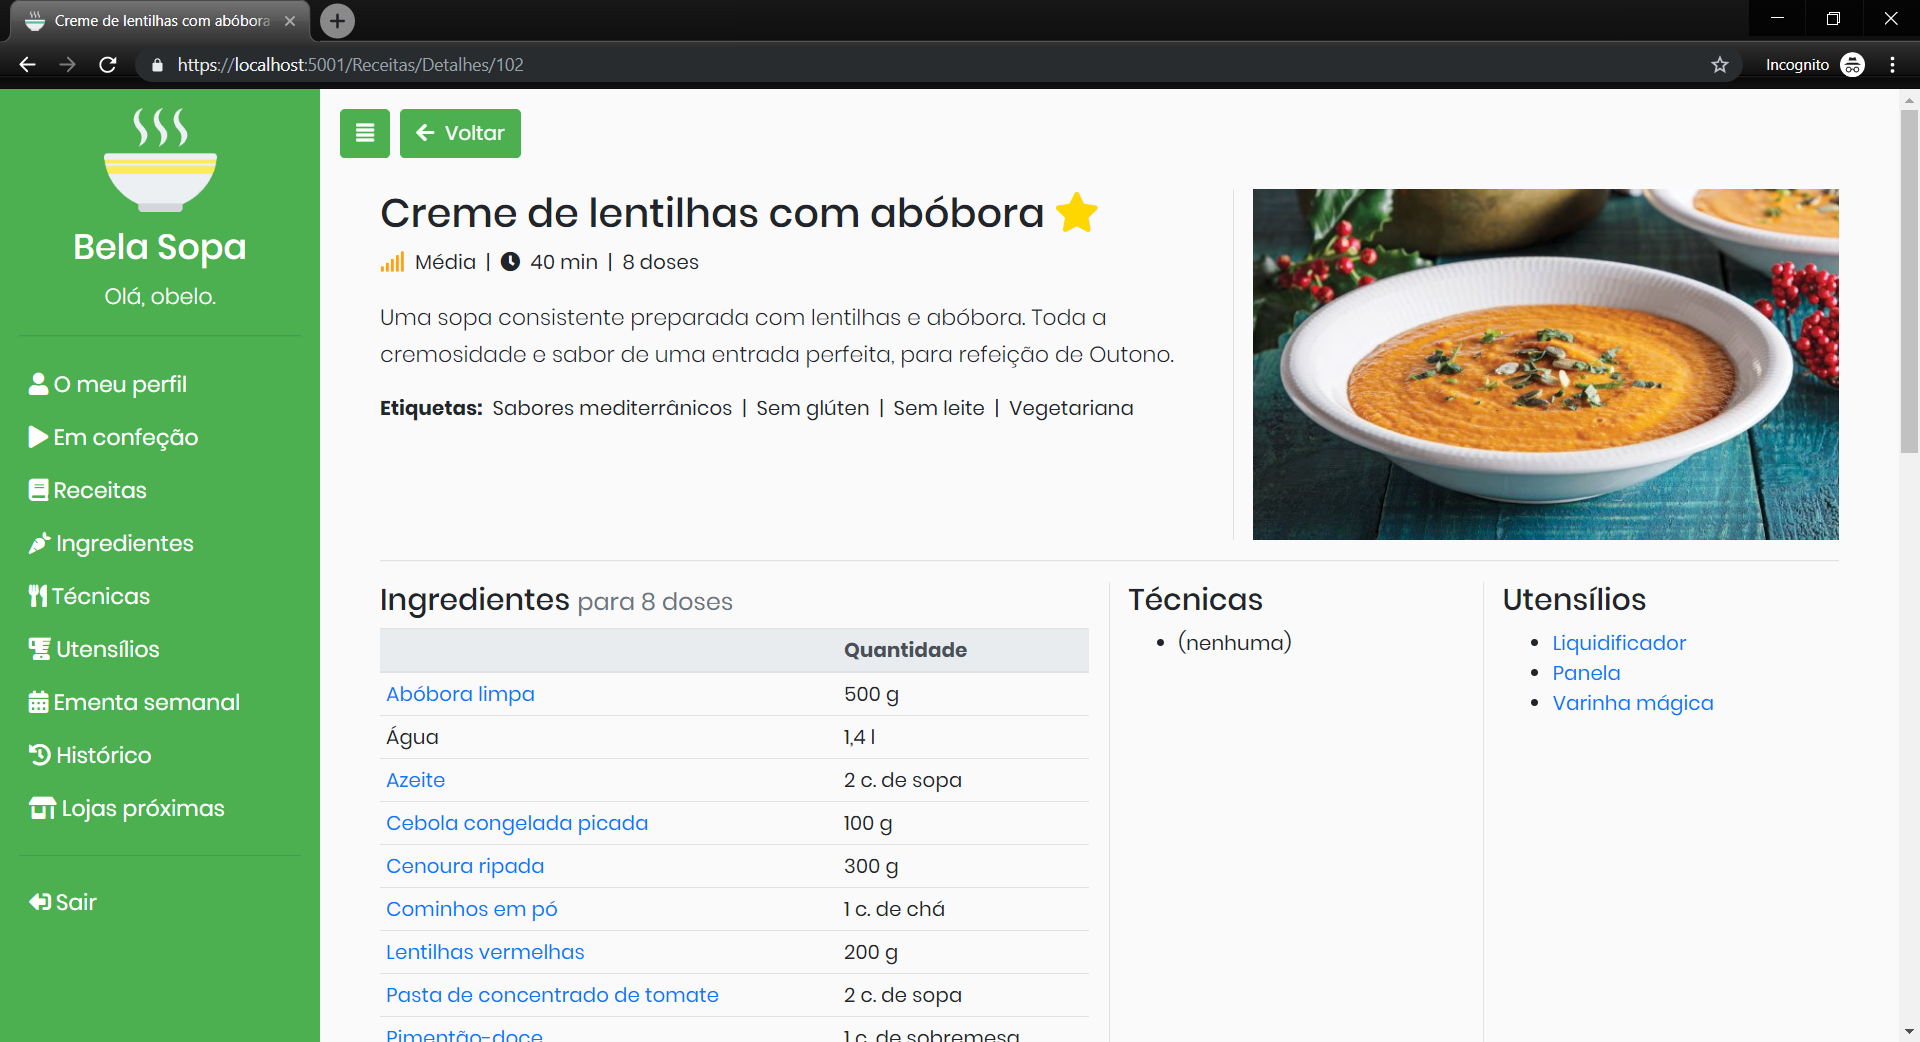
\includegraphics[height=.85\textheight]{figures/11/final-4.png}
  \caption{Aspeto final da interface de visualização de uma receita.}
  \label{fig:construcao:final-4}
\end{figure}

\end{landscape}

% ---------------------------------------------------------------------------- %
